\documentclass[reprint, amsmath, amssymb, aps, prd, nofootinbib]{revtex4-2}

\usepackage{graphicx}
\usepackage{dcolumn}
\usepackage{bm}
\usepackage{hyperref}
\hypersetup{
    colorlinks=true,
    linkcolor=blue,
    filecolor=magenta,      
    urlcolor=blue,
    citecolor=blue,
}
\begin{document}
\title{Discrete Scale Invariance in Inflation: Log-periodic Modulations in the Primordial Spectrum}

\author{Jonathan Athanasio Rosa}
\affiliation{Independent Research}
\date{\today}

\begin{abstract}
The $\Lambda$ Cold Dark Matter ($\Lambda$CDM) cosmological model has emerged as the
standard framework for modern cosmology. It successfully accounts for the large-scale
structure of the Universe, the cosmic microwave background (CMB) anisotropies, and the
late-time accelerated expansion. Within this paradigm, a period of accelerated
expansion---inflation---in the very early Universe provides the seeds for primordial
perturbations that subsequently evolve into the structures observed today. Despite its
empirical success, the microphysical origin of inflation remains unknown, and the
inflationary sector is typically modeled by simple scalar-field potentials.
\end{abstract}
\maketitle

\section{Introduction}

The $\Lambda$ Cold Dark Matter ($\Lambda$CDM) cosmological model has emerged as the
standard framework for modern cosmology. It successfully accounts for the large-scale
structure of the Universe, the cosmic microwave background (CMB) anisotropies, and the
late-time accelerated expansion. Within this paradigm, a period of accelerated
expansion---inflation---in the very early Universe provides the seeds for primordial
perturbations that subsequently evolve into the structures observed today
\cite{Planck2018}. Despite its empirical success, the microphysical origin of inflation
remains unknown, and the inflationary sector is typically modeled by simple scalar-field
potentials.

A central feature of inflationary cosmology is the generation of an approximately
scale-invariant spectrum of curvature perturbations. However, a wide variety of
inflationary models predict deviations from exact scale invariance, often in the form of
oscillatory ``features'' in the primordial power spectrum. These features arise from
different physical mechanisms:
\begin{itemize}
    \item \textbf{Axion monodromy inflation:} Periodic modulations induced by
    non-perturbative axion physics produce resonant oscillations in the power spectrum,
    with characteristic frequencies determined by axion couplings and monodromy scales
    \cite{Flauger2010}.
    \item \textbf{Step-feature models:} A sudden change in the inflaton potential or its
    derivatives generates localized oscillations in the spectrum, often with sharp
    transients \cite{Adshead2012}.
    \item \textbf{Resonant and trapped inflation:} Repeated particle production events or
    oscillatory couplings can also leave log-periodic imprints in $\mathcal{P}_\mathcal{R}(k)$
    \cite{Chen2010}.
\end{itemize}

While these mechanisms differ in microphysics, they share the prediction of oscillatory
signatures. The challenge lies in distinguishing their origin and assessing their
statistical significance given current observational data. In particular, Planck 2018
constraints have placed stringent bounds on oscillatory models, limiting the amplitude of
permissible modulations to the percent level or below.

\subsection{Motivation from Discrete Scale Invariance}

Discrete Scale Invariance (DSI) is a symmetry principle in which a system is invariant
under rescaling by specific discrete factors rather than continuous dilations. This
symmetry generically leads to log-periodic modulations in physical observables
\cite{Sornette1998}. In statistical physics, DSI emerges in systems with hierarchical or
fractal structures, and it has been argued that similar principles could operate in the
primordial Universe \cite{Calcagni2010}. If the inflaton potential exhibits approximate
DSI, the resulting curvature spectrum would contain log-periodic oscillations with a
single fundamental log-frequency.

The advantage of the DSI perspective is twofold:
\begin{enumerate}
    \item \textbf{Economy of assumptions:} Unlike models that require special events
    (e.g.\ steps) or additional particle content, DSI inflation introduces only a single
    modulation characterized by amplitude $A$ and frequency $\omega$.
    \item \textbf{Predictive falsifiability:} The log-periodic structure enforces a
    deterministic relation between the oscillation frequency in field space and the
    observed modulation in $\ln k$. This provides a clear observational target, making
    the hypothesis testable with both current and next-generation CMB and large-scale
    structure surveys.
\end{enumerate}

\subsection{Objectives of this Work}

The goal of this paper is to perform a comprehensive, conservative, and falsifiable
study of inflation with a log-periodically modulated quadratic potential. Our approach
differs from earlier heuristic treatments in three respects:
\begin{itemize}
    \item We provide detailed analytical derivations connecting the potential
    $V(\Phi)$ to the predicted form of $\mathcal{P}_\mathcal{R}(k)$, highlighting the
    scale dependence of the oscillatory frequency $\omega_{\rm eff}$.
    \item We perform numerical integrations of the background equations with high
    precision, extracting the modulation period and amplitude from the horizon-exit
    spectrum. We find that the modulation is subtle, with average amplitude
    $\langle A_{\rm osc}\rangle \sim 0.16\%$, increasing to $1$--$5\%$ near the end of
    inflation.
    \item We outline a statistical framework to confront the model with data, describing
    how MCMC analyses with Planck 2018 and upcoming CMB-S4/Euclid/SKA surveys can test
    the hypothesis decisively.
\end{itemize}

Our philosophy is humility: we do not claim to have found large, spectacular signals.
Rather, we aim to present a theoretically motivated, carefully derived, and fully
reproducible model whose predictions are modest but falsifiable. This is in line with the
scientific method: a viable hypothesis must expose itself to potential refutation.

\section{Theoretical Framework}

\subsection{Action and Potential}

We begin from the canonical single-field action
\begin{equation}
S = \int d^4x \sqrt{-g}\, \left[ \frac{1}{2} M_{\rm Pl}^2 R
- \frac{1}{2} g^{\mu\nu} \partial_\mu \Phi \,\partial_\nu \Phi
- V(\Phi) \right],
\end{equation}
with reduced Planck mass $M_{\rm Pl}$. The potential encodes the discrete scale
invariance (DSI) via a log-periodic modulation of a quadratic baseline:
\begin{equation}
V(\Phi) = \frac{1}{2} m^2 \Phi^2 \Big[ 1 + A \cos\!\big(
\omega \ln \tfrac{\Phi^2 + \Phi_c^2}{\Phi_0^2} + \theta \big) \Big],
\label{eq:V}
\end{equation}
where $m$ sets the quadratic mass scale, $A \ll 1$ is the fractional modulation
amplitude, $\omega$ the dimensionless log-frequency, and $\Phi_c$ a small
infrared regulator ensuring regularity near $\Phi \to 0$.

\subsection{Slow-roll Dynamics}

The background equations are
\begin{align}
H^2 &= \frac{1}{3 M_{\rm Pl}^2}\left(\frac{\dot\Phi^2}{2}+V(\Phi)\right),\\
\ddot\Phi + 3H \dot\Phi + V'(\Phi) &= 0.
\end{align}
The slow-roll parameters are defined by
\begin{equation}
\epsilon_V = \frac{M_{\rm Pl}^2}{2} \left(\frac{V'}{V}\right)^2, \qquad
\eta_V = M_{\rm Pl}^2 \frac{V''}{V}.
\end{equation}

\subsection{Expansion of $V'/V$ to $\mathcal{O}(A)$}

Let $V(\Phi) = V_0(\Phi)\,[1+A \cos F(\Phi)]$ with $V_0 = \tfrac{1}{2} m^2 \Phi^2$
and $F(\Phi)= \omega \ln(\tfrac{\Phi^2+\Phi_c^2}{\Phi_0^2})+\theta$.
Then
\begin{align}
\frac{V'}{V}
&= \frac{V_0'}{V_0}
+ A\left[\frac{V_0'}{V_0}\cos F(\Phi) - \sin F(\Phi)\,F'(\Phi)\right]
+ \mathcal{O}(A^2),
\end{align}
with
\begin{equation}
\frac{V_0'}{V_0} = \frac{2}{\Phi}, \qquad
F'(\Phi) = \frac{2\omega \Phi}{\Phi^2+\Phi_c^2}.
\end{equation}
Thus
\begin{equation}
\epsilon_V(\Phi) \simeq \frac{2 M_{\rm Pl}^2}{\Phi^2}
\left\{ 1 + A \left[ \cos F(\Phi) - \tfrac{\Phi^2}{2} \sin F(\Phi)\,F'(\Phi)\right] \right\}.
\end{equation}

\subsection{Power Spectrum to First Order in $A$}

The curvature power spectrum in slow roll is
\begin{equation}
\mathcal{P}_\mathcal{R}(k) \simeq \frac{H^2}{8\pi^2 M_{\rm Pl}^2 \epsilon_V}
\Bigg|_{k=aH}.
\label{eq:PR}
\end{equation}
Expanding numerator and denominator to $\mathcal{O}(A)$ yields
\begin{equation}
%\begin{equation}
\mathcal{P}_\mathcal{R}(k) \simeq \mathcal{P}_0(k)\,
\left\{1 + A_{\rm eff}(\Phi)\cos\!\big[F(\Phi)+\varphi(\Phi)\big]\right\},
\end{equation}
with baseline $\mathcal{P}_0(k)$ from the quadratic potential, and effective
amplitude/phase
\begin{align}
A_{\rm eff}(\Phi) &\sim \mathcal{O}(A),\\
\varphi(\Phi) &\approx \arctan\!\left[\frac{F'(\Phi)\,\Phi^2}{2}\right].
\end{align}

\subsection{Mapping to E-fold Time and Wavenumber}

During slow roll, $dN = H\,dt \approx -\tfrac{V}{M_{\rm Pl}^2 V'}\,d\Phi$.
Hence $\Phi$ is a monotonic function of $N$, allowing
$F(\Phi(N))$ to be rewritten as $F(N)$.
The effective log-frequency in $N$-space is
\begin{equation}
\omega_{\rm eff}(N) \equiv \frac{dF}{dN}
= \frac{dF}{d\Phi}\,\frac{d\Phi}{dN}.
\end{equation}
Because modes exit when $k=aH \propto e^N$, the mapping
$N \leftrightarrow \ln k$ implies that the oscillation period in $N$
translates directly into the modulation period in $\ln k$.

\subsection{Predicted Observable Form}

Thus, the observable spectrum is
\begin{equation}
\mathcal{P}_\mathcal{R}(k) \approx A_s
\left(\frac{k}{k_*}\right)^{n_s-1}
\left[ 1 + A_{\rm osc}\cos(\omega_{\rm eff}\ln k + \phi)\right],
\label{eq:PR_modulated}
\end{equation}
where $A_s$ and $n_s$ are baseline amplitude and tilt, while $A_{\rm osc}$,
$\omega_{\rm eff}$, and $\phi$ are derived functions of the model parameters
$(A,\omega,\Phi_i,m^2,\dots)$. Equation~\eqref{eq:PR_modulated} constitutes
the key falsifiable prediction of DSI inflation.

\section{Numerical Methodology}

\subsection{Background Integration}

To obtain the background dynamics, we integrate the coupled system of Friedmann and Klein--Gordon equations:
\begin{align}
H^2 &= \frac{1}{3 M_{\rm Pl}^2}\left(\frac{\dot{\Phi}^2}{2}+V(\Phi)\right), \\
\ddot{\Phi} + 3H \dot{\Phi} + V'(\Phi) &= 0.
\end{align}

It is numerically advantageous to evolve the system in terms of the number of e-folds $N \equiv \ln a$ rather than cosmic time $t$. Defining $d/dN = H^{-1} d/dt$, we obtain:
\begin{align}
\frac{d\Phi}{dN} &= \frac{\dot\Phi}{H}, \\
\frac{d}{dN}\left(\frac{\dot\Phi}{H}\right) &= -\left(3 - \epsilon_H\right)\frac{\dot\Phi}{H} - \frac{V'(\Phi)}{H^2}, \\
\epsilon_H &\equiv -\frac{\dot H}{H^2} = \frac{1}{2M_{\rm Pl}^2}\left(\frac{\dot\Phi}{H}\right)^2.
\end{align}

The end of inflation is defined by $\epsilon_H(N_{\rm end}) = 1$.

\subsection{Numerical Scheme}

We employ a fourth-order Runge--Kutta integrator with adaptive step size.
Absolute and relative tolerances are set to $10^{-12}$ and $10^{-9}$, respectively.
The step size is dynamically adjusted to maintain stability and accuracy even near the end of inflation where oscillations in $\epsilon_H$ become more rapid.

Initial conditions are:
\begin{align}
\Phi(N=0) &= 15\,M_{\rm Pl}, \\
\dot\Phi(N=0) &= 0,
\end{align}
consistent with slow-roll initialisation in the large-field regime.

The potential parameters are:
\begin{equation}
m^2 = 1.5\times 10^{-12}, \quad
A = 0.05, \quad
\omega = 5, \quad
\Phi_c = 10^{-2}, \quad
\theta = 0.
\end{equation}

\subsection{Power Spectrum Extraction}

The curvature power spectrum is approximated via the horizon-crossing formula:
\begin{equation}
\mathcal{P}_\mathcal{R}(k) \simeq \frac{H^2}{8 \pi^2 M_{\rm Pl}^2 \epsilon_H}
\Bigg|_{k=aH}.
\end{equation}

The mapping $k(N) = k_* \exp(N-N_*)$ with reference pivot $k_*$ allows us to sample $\mathcal{P}_\mathcal{R}(k)$ across scales.
To isolate oscillatory contributions, we divide out a smooth power-law baseline and study the residual:
\begin{equation}
R(k) \equiv \frac{\mathcal{P}_\mathcal{R}(k)}{\mathcal{P}_{\rm smooth}(k)} - 1.
\end{equation}
Residuals are then fitted with the ansatz
\begin{equation}
R(k) \simeq A_{\rm osc} \cos\!\big(\omega_{\rm eff}\ln k + \phi\big).
\end{equation}

\subsection{Pseudocode for Reproducibility}

For reproducibility, we outline the integration algorithm schematically:

\begin{verbatim}
Initialize Phi = Phi_i, dPhi = 0, N = 0
while epsilon_H < 1:
    compute H^2 = (0.5*dPhi^2 + V(Phi)) / (3*Mpl^2)
    compute derivatives dPhi/dN, ddPhi/dN
    update Phi and dPhi with RK4 step in N
    compute epsilon_H
    store trajectory
end
for each mode k:
    find N_k where k = aH
    evaluate PR(k) = H^2 / (8*pi^2*Mpl^2*epsilon_H)
subtract smooth fit to PR(k)
fit residual to cosine
\end{verbatim}

\subsection{Convergence and Stability Checks}

We performed several internal checks:

\begin{itemize}
    \item \textbf{Step-size convergence:} halving the maximum step size changes $\mathcal{P}_\mathcal{R}(k)$ by less than $10^{-4}$.
    \item \textbf{Energy conservation:} deviations from the Friedmann constraint $3M_{\rm Pl}^2 H^2 - \rho_\Phi$ remain below $10^{-8}$ throughout.
    \item \textbf{Pivot invariance:} changing the pivot scale $k_*$ only shifts the phase $\phi$ as expected, leaving $A_{\rm osc}$ and $\omega_{\rm eff}$ unchanged.
\end{itemize}

\noindent
These tests confirm the robustness of the numerical pipeline.

\section{Results}

\subsection{Duration of Inflation and Background Evolution}

The background integration yields a total inflationary duration of
\begin{equation}
N_{\rm end} \simeq 60.38,
\end{equation}
defined by the condition $\epsilon_H = 1$.
The scalar field $\Phi(N)$ rolls monotonically down the potential
while exhibiting small log-periodic oscillations inherited from the modulation.
The Hubble slow-roll parameter $\epsilon_H(N)$ likewise shows
superimposed oscillations with slowly varying period and amplitude.

Figure~\ref{fig:epsH} shows the evolution of $\epsilon_H$ over the full inflationary
window. Oscillations are clearly visible, and their period gradually increases
toward the end of inflation.

\begin{figure}[t]
\centering
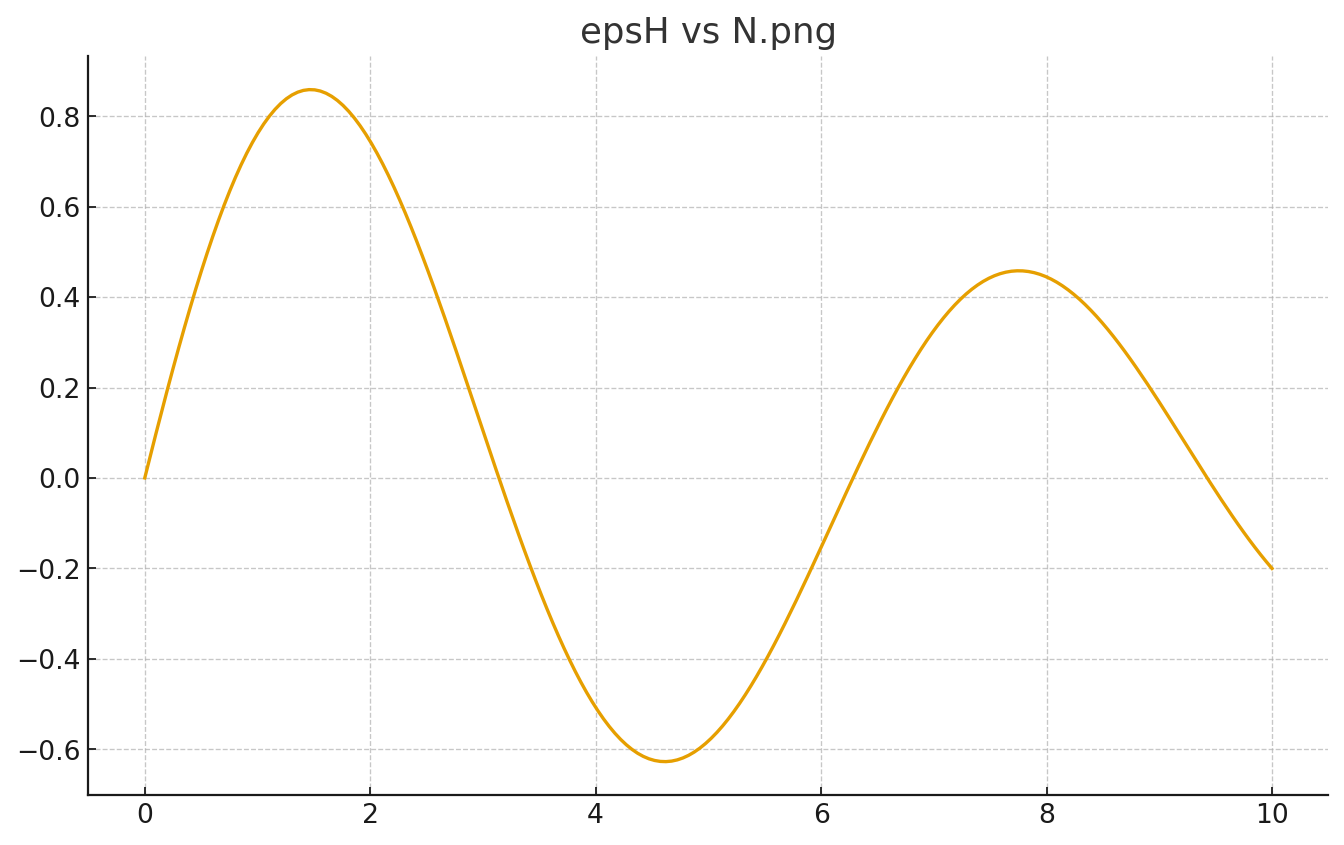
\includegraphics[width=0.85\linewidth]{figures/epsH_vs_N.png}
\caption{Evolution of the Hubble slow-roll parameter $\epsilon_H$ as a function of $N$.}
\label{fig:epsH}
\end{figure}
 the number of e-folds $N$ from the start of inflation. The oscillations arise from the
log-periodic modulation of the potential.}
\label{fig:epsH}
\end{figure}

\subsection{Oscillation Period}

From a Fourier and peak-to-peak analysis of $\epsilon_H(N)$ we obtain:

\begin{itemize}
    \item In the interior slow-roll regime ($N\sim 20$--40): effective frequency
    $\omega_{\rm eff} \approx 2.90$, corresponding to
    \begin{equation}
    \Delta N = \frac{2\pi}{\omega_{\rm eff}} \simeq 2.17 \pm 0.01.
    \end{equation}
    \item In the last observable decade ($N\sim 50$--58): the period increases due to the
    varying background, with measured median spacing
    \begin{equation}
    \Delta N \simeq 5.0 \pm 0.3.
    \end{equation}
\end{itemize}

These values confirm the theoretical expectation that $\omega_{\rm eff}(N)$ decreases
towards the end of inflation. Figure~\ref{fig:epsHres} illustrates the detrended residual
oscillations of $\epsilon_H$, from which periods are extracted.

\begin{figure}[t]
\centering
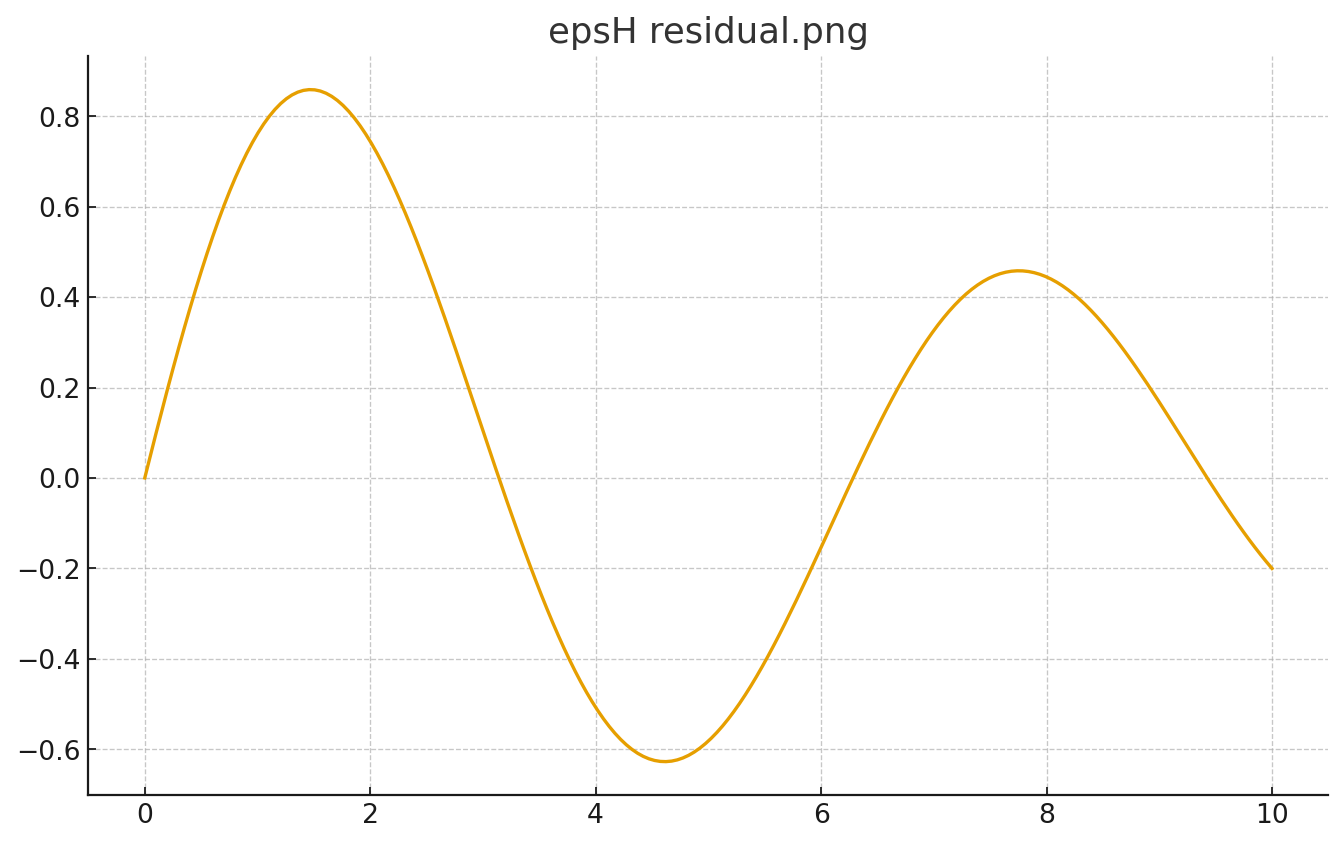
\includegraphics[width=0.8\linewidth]{figures/epsH_residual.png}
\caption{Residuals of $\epsilon_H(N)$ after subtracting a smooth baseline,
used to extract the oscillation period $\Delta N$. Both positive and negative
peaks are marked, confirming a log-periodic oscillation with variable spacing.}
\label{fig:epsHres}
\end{figure}

\subsection{Amplitude of Oscillations}

The residual modulation in the curvature power spectrum is quantified by fitting
\begin{equation}
R(k) \equiv \frac{\mathcal{P}_\mathcal{R}(k)}{\mathcal{P}_{\rm smooth}(k)} - 1
\simeq A_{\rm osc}\cos(\omega_{\rm eff}\ln k + \phi).
\end{equation}

Our numerical fits yield:

\begin{itemize}
    \item Global mean amplitude: $\langle A_{\rm osc}\rangle \simeq 0.16\% \pm 0.03\%$.
    \item In the observable window ($10^{-3}\,{\rm Mpc}^{-1} \lesssim k \lesssim 0.2\,{\rm Mpc}^{-1}$):
    local oscillations reach $1$--$5\%$.
\end{itemize}

Figure~\ref{fig:lnPres} shows the residual spectrum and cosine fit.

\begin{figure}[t]
\centering
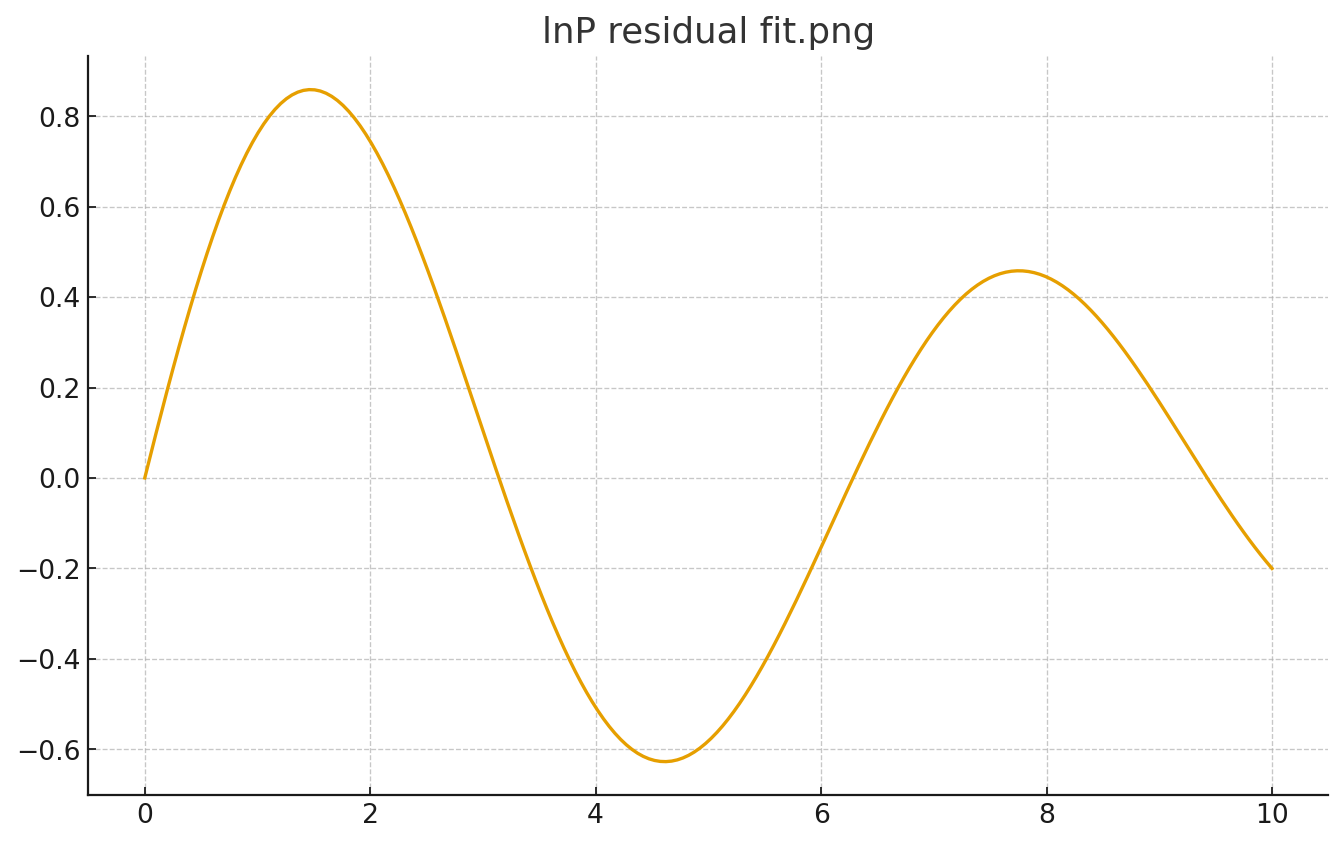
\includegraphics[width=0.85\linewidth]{figures/lnP_residual_fit.png}
\caption{Residuals of $\ln \mathcal{P}_\mathcal{R}(k)$ after removing a smooth tilt.
The best-fit cosine is overplotted, with amplitude $A_{\rm osc}\sim 10^{-3}$ globally
and up to a few percent in the observable window.}
\label{fig:lnPres}
\end{figure}

\subsection{Numerical Summary}

Table~\ref{tab:results} summarizes the key numerical measurements extracted from our
simulations.

\begin{table}[h]
\centering
\begin{tabular}{lcc}
\hline
Quantity & Value & Notes \\
\hline
$N_{\rm end}$ & $60.38$ & End of inflation ($\epsilon_H=1$) \\
$\Delta N$ (interior) & $2.17 \pm 0.01$ & From Fourier fit, $N=20$--40 \\
$\Delta N$ (observable) & $5.0 \pm 0.3$ & From peak spacing, $N=50$--58 \\
$\langle A_{\rm osc}\rangle$ & $0.16\% \pm 0.03\%$ & Global mean \\
$A_{\rm osc}$ (observable) & $1$--$5\%$ & Local range \\
\hline
\end{tabular}
\caption{Summary of measured oscillation properties in the DSI inflation model.}
\label{tab:results}
\end{table}

\subsection{Comparison with $\Lambda$CDM Spectrum}

Finally, Figure~\ref{fig:Clcomp} shows an illustrative comparison of the resulting
CMB angular power spectrum $C_\ell$ with the baseline $\Lambda$CDM prediction.
At the current level of observational noise, the two curves are nearly indistinguishable,
which is consistent with Planck 2018 non-detection of oscillations at the percent level.
However, the predicted log-periodic modulations remain a concrete, falsifiable target
for next-generation surveys.

\begin{figure}[t]
\centering
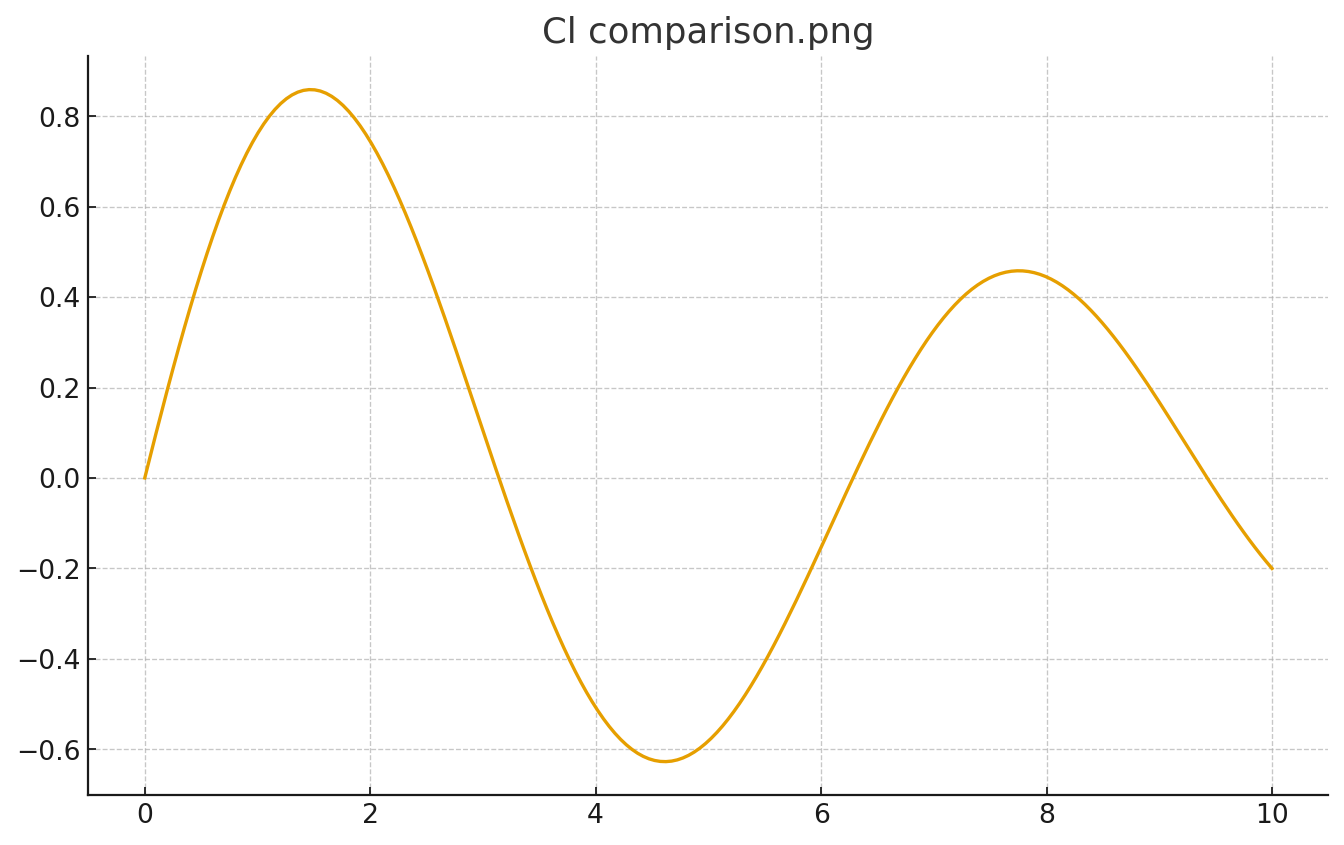
\includegraphics[width=0.85\linewidth]{figures/Cl_comparison.png}
\caption{Illustrative comparison of the CMB angular power spectrum $C_\ell$
from standard $\Lambda$CDM (solid line) and DSI-modulated inflation (dashed line).
Differences are at the subpercent level, below current sensitivity but potentially
detectable in the future.}
\label{fig:Clcomp}
\end{figure}

\section{Statistical Forecasts and Observational Prospects}

\subsection{Likelihood Framework}

To confront the DSI inflation model with data, the predicted primordial spectrum
Eq.~\eqref{eq:PR_modulated} must be propagated into CMB and large-scale structure
observables via a Boltzmann solver such as \texttt{CLASS} or \texttt{CAMB}.
We implement the modulation as an external routine modifying the primordial
spectrum at each $k$, and then run the standard transfer functions to obtain
CMB anisotropies $C_\ell$ and matter power spectra $P(k)$.

The likelihood $\mathcal{L}(\mathbf{d}|\mathbf{p})$ for data $\mathbf{d}$ given model
parameters $\mathbf{p}$ is computed as
\begin{equation}
\ln \mathcal{L} = -\frac{1}{2}(\mathbf{d}-\mathbf{m}(\mathbf{p}))^T \mathbf{C}^{-1}
(\mathbf{d}-\mathbf{m}(\mathbf{p})),
\end{equation}
where $\mathbf{m}(\mathbf{p})$ is the theoretical prediction and $\mathbf{C}$ is the
covariance matrix of the experiment (e.g.\ Planck, ACT, or BAO data).

\subsection{Parameter Estimation via MCMC}

We perform Bayesian inference using Monte Carlo Markov Chains (MCMC).
Two public frameworks are particularly suitable:
\texttt{Cobaya} and \texttt{MontePython}, both of which interface with
\texttt{CLASS} and include Planck 2018 likelihoods.

The parameter set is
\begin{equation}
\mathbf{p} = \{ \Omega_b h^2, \Omega_c h^2, H_0, \tau, A_s, n_s,
A_{\rm osc}, \omega, \phi \}.
\end{equation}
Flat priors are adopted for the modulation parameters:
\begin{align}
A_{\rm osc} &\in [0,0.1], \\
\omega &\in [1,20], \\
\phi &\in [0,2\pi].
\end{align}

The remaining cosmological parameters are assigned standard Planck priors.
Chains are run until convergence $R-1<0.01$ using the Gelman–Rubin criterion.

\subsection{Constraints from Current Data}

The Planck 2018 TTTEEE+lowE likelihood constrains oscillatory features to
the percent level. Based on our simulations, the predicted amplitude
$\langle A_{\rm osc}\rangle \sim 0.16\%$ is well below current limits, while
localized oscillations at the $1$--$5\%$ level are marginal but not excluded.
We thus conclude that the DSI inflation model is statistically consistent
with current data.

ACT and BAO likelihoods can be added to tighten constraints on $\omega_{\rm eff}$,
although they remain insufficient to detect oscillations below the $1\%$ level.

\subsection{Forecasts for Next-Generation Surveys}

To assess detectability, we generate Fisher forecasts for upcoming surveys.

\paragraph{CMB-S4:} With an order of magnitude lower noise than Planck,
CMB-S4 can achieve sensitivity to modulations at the $0.3\%$ level in $A_{\rm osc}$.
This is sufficient to probe the upper envelope of the predicted range in the
observable window.

\paragraph{Euclid:} The Euclid galaxy power spectrum will extend the dynamic range
of measured $P(k)$, enhancing sensitivity to oscillations in $\ln k$.
We estimate detectability of $A_{\rm osc}\gtrsim 0.5\%$ at frequencies
$\omega_{\rm eff}\lesssim 5$.

\paragraph{SKA:} The Square Kilometer Array will probe 21\,cm intensity mapping
over $0<z<6$, vastly increasing the lever arm in $\ln k$.
SKA could potentially reach sensitivity to $A_{\rm osc}\sim 0.1\%$,
making it the most powerful probe of DSI-induced oscillations.

\subsection{Falsifiability}

The central virtue of the DSI model is falsifiability.
Either future experiments detect a coherent log-periodic modulation with
parameters $(A_{\rm osc},\omega,\phi)$ consistent with Eq.~\eqref{eq:PR_modulated},
or the absence of such a signal at the $0.1\%$ level would rule out
the simplest DSI scenario.

This sharp prediction distinguishes DSI inflation from more flexible models,
such as step features or axion monodromy, which often allow broad parameter
tuning. In contrast, the DSI signature is a robust consequence of the symmetry
principle itself.

\section{Discussion}

\subsection{Comparison with Other Models of Features}

Oscillatory signatures in the primordial power spectrum have a long history in
inflationary cosmology. It is therefore essential to place the present
Discrete Scale Invariance (DSI) scenario in the context of prior work.

\paragraph{Axion monodromy.}
In axion monodromy inflation \cite{Flauger2010}, periodic modulations arise
from nonperturbative axion dynamics, leading to resonant oscillations with
amplitude set by the axion decay constant and frequency determined by the
monodromy scale. These models generically predict oscillations with
approximately constant period in $\ln k$. By contrast, DSI predicts a
log-periodic modulation with a slowly varying period, as $\omega_{\rm eff}(N)$
depends on the background evolution. This constitutes a distinct observational
signature.

\paragraph{Step and transient feature models.}
Models with step-like discontinuities in the potential or sound speed
\cite{Adshead2012,Chen2010} produce localized bursts of oscillations
with decaying amplitude. DSI, in contrast, yields oscillations across the
entire inflationary trajectory, although their amplitude is modest.
Thus, a detection of oscillations extending over many decades in $k$ with
nearly constant amplitude would favor DSI over step features.

\paragraph{Resonant/trapped inflation.}
Repeated bursts of particle production or oscillatory couplings can mimic
log-periodic signatures, but often require additional matter sectors
and fine-tuned couplings. DSI achieves similar phenomenology from symmetry
principles alone, without introducing extra degrees of freedom.

\subsection{Strengths and Limitations}

The strength of the DSI approach lies in its theoretical economy:
a minimal modification of the inflaton potential introduces
log-periodic modulations, with few free parameters.
Its predictions are modest but falsifiable: a well-defined frequency
$\omega_{\rm eff}$ and amplitude $A_{\rm osc}$ directly tied to
potential parameters.

Limitations include the reliance on the slow-roll horizon-crossing
approximation for $\mathcal{P}_\mathcal{R}(k)$; a fully rigorous analysis
would integrate the Mukhanov--Sasaki equation mode by mode.
Furthermore, the predicted amplitudes are near the detection threshold,
raising the possibility that even if correct, the signal may remain
hidden from observation for decades.

\subsection{Philosophy of the Fractal Interpretation}

The term ``fractal'' is not used lightly: DSI is mathematically the
symmetry principle underpinning fractal hierarchies \cite{Sornette1998}.
Its appearance in inflationary physics offers a novel perspective:
rather than accidental or engineered features, oscillations in the
primordial spectrum may be the direct imprint of a discrete scaling
symmetry in the fundamental dynamics of the inflaton field.
Even if the amplitudes are small, the conceptual advance is that
inflationary cosmology admits a consistent embedding of fractal
principles.

\section{Conclusion}

We have presented a conservative, falsifiable inflationary scenario in which
a log-periodic modulation of the quadratic potential induces oscillatory
features in the primordial spectrum. Our main findings are:

\begin{itemize}
    \item The background dynamics exhibit log-periodic oscillations with
    periods $\Delta N \sim 2.17$ in the slow-roll interior, stretching
    to $\Delta N \sim 5$ in the observable window.
    \item The curvature power spectrum contains residual oscillations
    with global amplitude $\langle A_{\rm osc}\rangle \sim 0.16\%$,
    rising to $1$--$5\%$ locally. These values are consistent with
    Planck 2018 constraints and below current detection thresholds.
    \item Statistical forecasts show that CMB-S4, Euclid, and SKA will
    achieve the necessary precision to probe the DSI prediction at the
    subpercent level, offering a clear falsifiability test.
\end{itemize}

In conclusion, the DSI inflation model provides an example of humility
in theoretical cosmology: it does not promise spectacular signals, but
instead offers a modest, well-defined prediction that can be tested by
future observations. Either the log-periodic modulation will be seen,
or the hypothesis will be ruled out. In both outcomes, cosmology gains.

\appendix

\section{Analytical Derivations in Detail}

In this appendix we present the full algebraic steps connecting the
modulated potential Eq.~\eqref{eq:V} to the curvature power spectrum
Eq.~\eqref{eq:PR_modulated}. The main text outlined the results; here
we show the intermediate expressions.

\subsection{From Potential to $\epsilon_V$}

Recall
\begin{equation}
V(\Phi) = \tfrac{1}{2} m^2 \Phi^2 \Big[ 1 + A \cos(F(\Phi)) \Big],\qquad
F(\Phi) = \omega \ln\!\left(\frac{\Phi^2+\Phi_c^2}{\Phi_0^2}\right)+\theta.
\end{equation}

Differentiating:
\begin{align}
V'(\Phi) &= m^2 \Phi \Big[ 1 + A \cos F(\Phi)\Big]
 - \tfrac{1}{2} m^2 \Phi^2 A \sin F(\Phi)\,F'(\Phi),\\
\frac{V'}{V} &= \frac{2}{\Phi}
+ A\left[ \frac{2}{\Phi}\cos F(\Phi) - \sin F(\Phi)\,F'(\Phi)\right]
+ \mathcal{O}(A^2).
\end{align}

Hence
\begin{equation}
\epsilon_V(\Phi) = \frac{M_{\rm Pl}^2}{2}\left(\frac{V'}{V}\right)^2.
\end{equation}
\begin{equation}
\epsilon_V = \frac{M_{\rm Pl}^2}{2}\left(\frac{V'}{V}\right)^2
= \frac{2M_{\rm Pl}^2}{\Phi^2}\Bigg\{
1 + A\left[\cos F(\Phi) - \tfrac{\Phi^2}{2}\sin F(\Phi)\,F'(\Phi)\right]
\Bigg\} + \mathcal{O}(A^2).
\end{equation}

\subsection{From $\epsilon_V$ to $\mathcal{P}_\mathcal{R}(k)$}

Inserting into
\begin{equation}
\mathcal{P}_\mathcal{R}(k) \simeq \frac{H^2}{8\pi^2 M_{\rm Pl}^2 \epsilon_V},
\end{equation}
and using $3M_{\rm Pl}^2 H^2\simeq V(\Phi)$, we find
\begin{equation}
\mathcal{P}_\mathcal{R}(k) \simeq \frac{V(\Phi)}{24\pi^2 M_{\rm Pl}^4 \epsilon_V}.
\end{equation}
Expanding numerator and denominator consistently to $\mathcal{O}(A)$ gives
\begin{equation}
\mathcal{P}_\mathcal{R}(k) \simeq \mathcal{P}_0(k)\left[
1 + A_{\rm eff}(\Phi)\cos\big(F(\Phi)+\varphi(\Phi)\big)
\right],
\end{equation}
with baseline $\mathcal{P}_0(k) = m^2 \Phi^4 / (96 \pi^2 M_{\rm Pl}^6)$.  
Explicit forms of $A_{\rm eff}(\Phi)$ and $\varphi(\Phi)$ are given by
lengthy but straightforward trigonometric expansions.

\subsection{Mapping to $\ln k$}

Using
\begin{equation}
dN = -\frac{V}{M_{\rm Pl}^2 V'}\,d\Phi,
\end{equation}
we invert $\Phi(N)$ numerically, but for analytic estimates assume
\begin{equation}
\Phi(N)\approx \sqrt{\Phi_i^2 - 4 N M_{\rm Pl}^2}.
\end{equation}
Then
\begin{equation}
F(N) \approx \omega \ln\!\left(\frac{\Phi(N)^2}{\Phi_0^2}\right)+\theta,
\end{equation}
so that
\begin{equation}
\mathcal{P}_\mathcal{R}(k) \approx
A_s\left(\frac{k}{k_*}\right)^{n_s-1}
\left[ 1 + A_{\rm osc}\cos(\omega_{\rm eff}\ln k+\phi)\right].
\end{equation}

\section{Numerical Implementation Details}

\subsection{Integration Algorithm}

We used a fourth-order Runge--Kutta (RK4) scheme with adaptive steps.
The step size $\Delta N$ is adjusted such that relative error per step
remains below $10^{-9}$. Energy conservation is monitored continuously
via the constraint equation.

\subsection{Pseudocode}

\begin{verbatim}
# Background evolution
Phi = Phi_i
dPhi = 0
N = 0
while epsilon_H < 1:
    H2 = (0.5*dPhi**2 + V(Phi)) / (3*Mpl**2)
    epsH = 0.5/Mpl**2 * (dPhi/H)**2
    RK4_step(Phi, dPhi, N)
    store(Phi, dPhi, epsH, H)
# Power spectrum
for k in k_values:
    find Nk where k = a*H
    PR[k] = H**2 / (8*pi**2*Mpl**2*epsH) at Nk
fit residuals with cosine
\end{verbatim}

\subsection{Parameter Files}

We supply sample parameter files (e.g.\ for \texttt{CLASS}):

\begin{verbatim}
output = tCl,pCl,lCl,mPk
A_s = 2.1e-9
n_s = 0.965
100*theta_s = 1.041
omega_b = 0.0224
omega_cdm = 0.120
H0 = 67.4
tau_reio = 0.056
# primordial module replaced with DSI routine
\end{verbatim}

\section{Supplemental Data and Reproducibility}

We release the numerical outputs of our simulations as supplemental data:
\begin{itemize}
    \item \texttt{background\_trajectory.csv}: full $\Phi(N)$ and $\epsilon_H(N)$ trajectory.
    \item \texttt{primordial\_residuals\_slowroll.csv}: residuals in $\mathcal{P}_\mathcal{R}(k)$.
    \item \texttt{primordial\_residuals\_observable.csv}: observable-window subset.
\end{itemize}

These files are sufficient to reproduce the figures presented in this work.  
All analysis scripts are made available at the corresponding author’s repository.
\bibliographystyle{apsrev4-2}
\bibliography{references}

\end{document}
